
\noindent
\begin{tabular}{cc}
\begin{minipage}{0.60\textwidth}
%\sectionIf{\flagSect}{\taitol{Esercizio}}
\begin{exercise}[Stevino: serbatoi]
Si consideri il sistema rappresentato in figura in cui un recipiente
aperto all'atmosfera, contenente olio con densit\`a $\rho= 800\ kg/m^3$, \`e
collegato tramite una tubazione a un secondo recipiente, contenente a
sua volta olio e aria non miscelati. Date le due altezze $h_1=1.5\ m$ e $h_2= 1.8 \ m$
del pelo libero nei due recipienti e l'altezza $H= 2.5\ m$ della tubatura,
determinare il valore della pressione nei punti A e B in figura,
esprimendolo sia in Pascal sia in metri d'acqua. Considerare la
pressione atmosferica standard ($101325\ Pa$).\\ 
($p_A=93477\ Pa = 9.53\ m_{H_2O}$, $p_B=98970.6\ Pa=10.10\ m_{H_2O}$.)
\end{exercise}
\end{minipage}
&
\begin{minipage}{0.35\textwidth}
   \begin{center}
   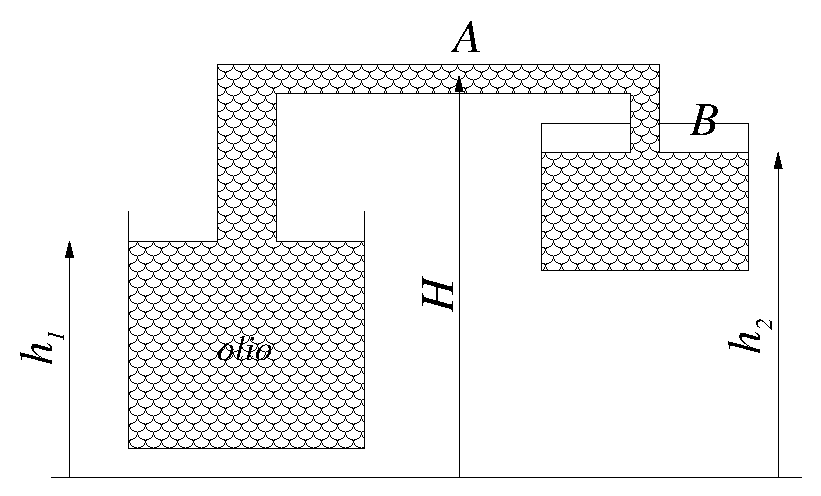
\includegraphics[width=0.90\textwidth]{./fig/recipientiariaolio.eps}
   \end{center}
\end{minipage}
\end{tabular}

\sol

\partone
Legge di Stevino, $P_1 + \rho g h_1 = P_2 + \rho g h_2 $.
%
Conversione $Pa$ - metri di $H_2O$, 
\begin{equation}
1 m_{{H_2O}} = P[Pa] = \rho_{H_2O} \cdot g \cdot 1 m =
9810 \dfrac{kg}{m^2 s^2} \cdot 1 m = 9810 Pa \ . 
\end{equation}

\parttwo
 Il problema si risolve applicando due volte la legge di Stevino e la conversione da Pascal $Pa$ a metri d'acqua $m_{H_2O}$.
Sia $O$ il punto sul pelo libero nel serbatoio \textit{aperto} di sinistra, sul quale agisce la pressione ambiente.

\begin{equation}
\begin{cases}
  P_A = P_O + \rho g (h_1 - H)  = 93477 Pa = \dfrac{93477}{9810} m_{H_2O} = 9.53 m_{H_2O}  & \text{(Stevino O-A)} \\ \\
  P_B = P_O + \rho g (h_1 - h_2) = 98970.6 Pa = \dfrac{98970.6}{9810} m_{H_2O}= 10.10 m_{H_2O} & \text{(Stevino O-B)}
\end{cases}
\end{equation}

